\documentclass[twoside]{article}
\usepackage{amssymb}
\usepackage{amsthm}
\usepackage{amsmath}
\usepackage{amsfonts}
\usepackage[utf8]{inputenc}
\usepackage[spanish]{babel}
\usepackage{tikz}
\usepackage{centernot}
\usepackage{hyperref}
\usepackage{fancyhdr}
\usepackage{lipsum}
\usepackage{subcaption}
\hypersetup{
    colorlinks,
    citecolor=black,
    filecolor=black,
    linkcolor=black,
    urlcolor=black
}
\usepackage{xurl}
\usepackage[top=1in, bottom=1.5in, left=1in, right=1in]{geometry}
\pagestyle{fancy}
\fancyhead{}
\fancyhead[L]{\leftmark}
\fancyfoot{}
\fancyfoot[C]{\thepage}
\newcommand{\enquote}[1]{``#1''}
\usepackage{float}
\usepackage[parfill]{parskip}
\newcommand{\image}[2]{
\begin{figure}[H]
    \includegraphics[width=#1 cm]{../images/#2.png}
    \centering
\end{figure}
}

\title{Práctica 2 SWAP}
\author{XuSheng Zheng}
\date{}

\begin{document}

\maketitle
\tableofcontents
\newpage

\section{Copia de archivos}
En primer lugar vamos a crear un un directorio local:
\image{8}{1}
Vamos a mandar este directorio a m2 mediante \textbf{tar} y \textbf{ssh}:
\image{8}{2}
Comprobamos descomprimiento el archivo tar:
\image{8}{3}
Esto también lo podemos llevar a cabo mediante scp, puesto que habíamos configurado \textbf{SSH} en el puerto 2222, necesitamos indicarlo con el argumento \textbf{-P}:
\image{8}{4}

\section{rsync}
En este apartado vamos a utilizar \textbf{rsync} para sincronizar ambas máquinas (de m1 a m2). En este caso, la herramienta ya esta instalada por defecto. En primer lugar, necesitamos dar privilegio a los usuarios sobre la carpeta donde están los archivos del servidor web:
\image{6}{5}
Para probar, vamos a sincronizar la carpeta anterior:
\image{8}{7}
Podemos ver que en este caso no ha sido posible transferir la carpeta porque no tenemos permiso para escribir sobre ella. Si examinamos la carpeta \textit{/var} en m2:
\image{8}{8}
nos damos cuenta de que sólo root tiene permiso para escribir sobre ella. Podemos retorgar el permiso al usuario en m2 también:
\image{6}{6}
Y volvemos a intentar:
\image{8}{9}
podemos ver que ahora sí se ha sincronizado correctamente.
\subsection{Opciones avanzadas}
En la sincronización que hemos visto anteriormente se ha utilizado los siguientes argumentos:
\begin{itemize}
    \item \textbf{-a}: la transferencia se realiza en modo archivo, lo que asegura que los permisos, atributos, enlaces, etc se preserven y que la transferencia sea recursiva.
    \item \textbf{-v}: modo verbose, para dar más información.
    \item \textbf{-z}: comprime los archivos durante la transferencia.
    \item \textbf{-e}: determina el shell remoto a utilizar.
\end{itemize}
Como opciones avanzadas vamos a utilizar \textbf{--exclude} para excluir que se copie la carpeta \textit{/var/www/img} que vamos a crear, además vamos a copiar un archivo txt en \textit{/var/www} para eliminarlo después:
\image{8}{10}
Podemos ver que ha excluido la carpeta \textit{/var/www/img} de la sincronización y sólo ha sincronizado el archivo txt. Ahora vamos a eliminar este archivo txt y probar con la opción \textbf{--delete}:
\image{8}{11}
Podemos ver que como se ha eliminado el archivo en la máquina origen, también se ha borrado en la máquina destino.




























\iffalse
\section{Instalación de máquinas virtuales}
Comenzamos con la instalación de las máquinas virtuales. Puesto que vamos a hacer lo mismo en ambas máquinas, vamos a centrarnos en la configuración de una de ellas:
\image{8}{1}
Le damos 4GB de RAM y 10 GB de disco duro:
\begin{figure}[H]
    \centering
    \begin{subfigure}{.5\textwidth}
        \centering
        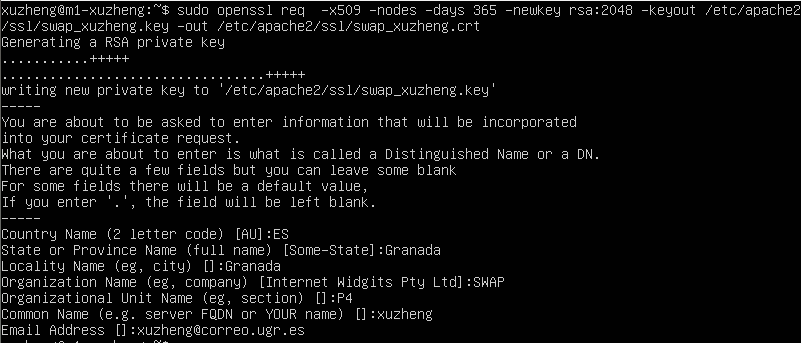
\includegraphics[width=7cm]{../images/2.png}
    \end{subfigure}%
    \begin{subfigure}{.5\textwidth}
        \centering
        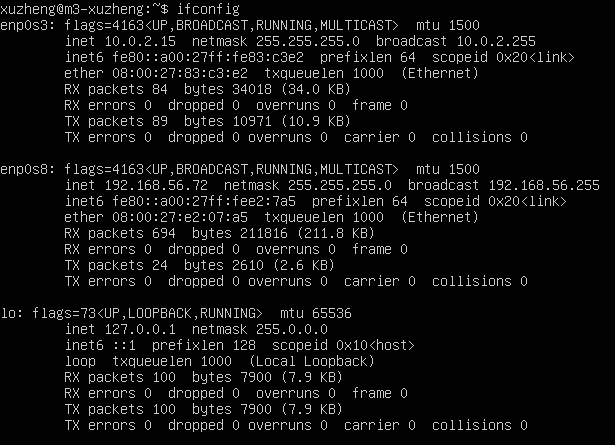
\includegraphics[width=7cm]{../images/3.png}
    \end{subfigure}
\end{figure}
\fi

\newpage
\section{Bibliografía}
\begin{itemize}
    \item \url{https://linux.die.net/man/1/scp}
    \item \url{https://linux.die.net/man/1/tar}
    \item \url{https://serverfault.com/questions/141773/what-is-archive-mode-in-rsync}
    \item \url{https://ss64.com/bash/rsync.html}
    \item \url{https://linux.die.net/man/1/rsync}
    

    \item \url{https://www.ionos.com/help/server-cloud-infrastructure/getting-started/important-security-information-for-your-server/changing-the-default-ssh-port/}
    \item \url{https://www.ibm.com/support/pages/configuring-ssh-login-without-password}
\end{itemize}

\end{document}
